\section{Figure Class Reference}
\label{classFigure}\index{Figure@{Figure}}
{\tt \#include $<$figure.h$>$}

Inheritance diagram for Figure::\begin{figure}[H]
\begin{center}
\leavevmode
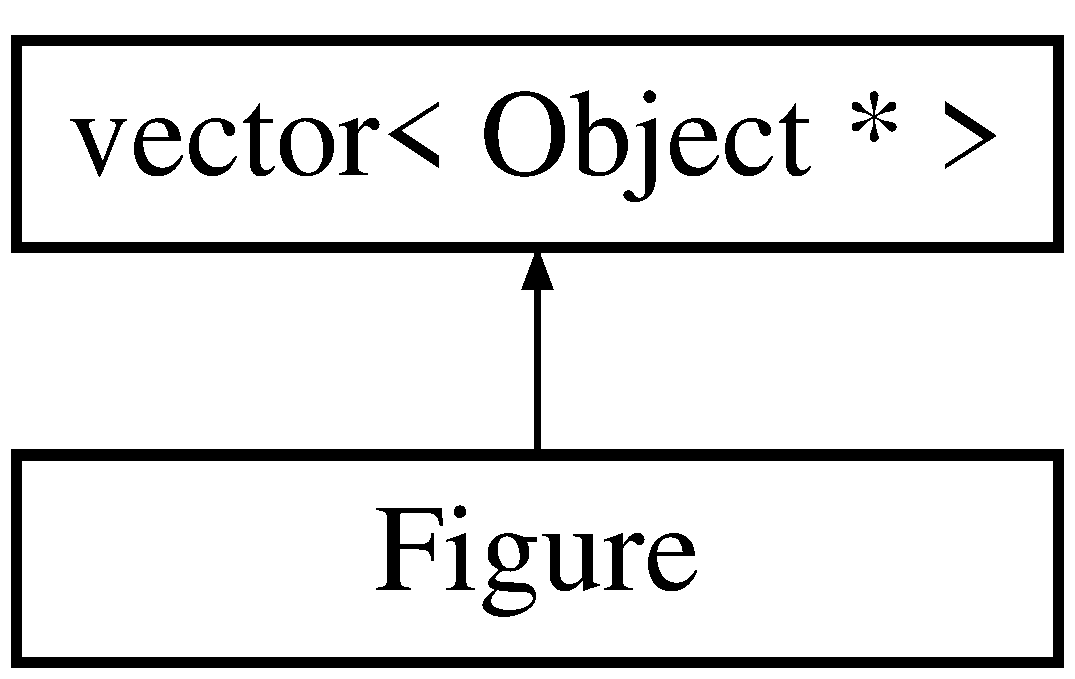
\includegraphics[height=2cm]{classFigure}
\end{center}
\end{figure}
\subsection*{Public Types}
\begin{CompactItemize}
\item 
enum {\bf Orientations} \{ {\bf Landscape} =  0, 
{\bf Portrait} =  1
 \}
\item 
enum {\bf Justifications} \{ {\bf Center} =  0, 
{\bf Flush\-Left} =  1
 \}
\item 
enum {\bf Units} \{ {\bf Metric} =  0, 
{\bf Inches} =  1
 \}
\item 
enum {\bf Papersizes} \{ {\bf Letter} =  0, 
{\bf Legal} =  1, 
{\bf Ledger} =  2, 
{\bf Tabloid} =  3, 
{\bf A} =  4, 
{\bf B} =  5, 
{\bf C} =  6, 
{\bf D} =  7, 
{\bf E} =  8, 
{\bf A4} =  9, 
{\bf A3} =  10, 
{\bf A2} =  11, 
{\bf A1} =  12, 
{\bf A0} =  13, 
{\bf B5} =  14
 \}
\item 
enum {\bf Multiple\-Pages} \{ {\bf Single} =  0, 
{\bf Multiple} =  1
 \}
\end{CompactItemize}
\subsection*{Public Methods}
\begin{CompactItemize}
\item 
{\bf Figure} ()
\item 
{\bf $\sim$Figure} ()
\item 
void {\bf set\-Orientation} ({\bf Orientations} {\bf orientation})
\item 
void {\bf set\-Justification} ({\bf Justifications} {\bf justification})
\item 
void {\bf set\-Units} ({\bf Units} {\bf units})
\item 
void {\bf set\-Papersize} ({\bf Papersizes} {\bf papersize})
\item 
void {\bf set\-Magnification} (float {\bf magnification})
\item 
void {\bf set\-Multiple\-Page} ({\bf Multiple\-Pages} {\bf multiple\-Page})
\item 
void {\bf set\-Transparent\-Color} (int {\bf transparent\-Color})
\item 
void {\bf set\-Resolution} (int {\bf resolution})
\item 
void {\bf set\-Coord\-System} (int {\bf coord\-System})
\item 
{\bf Orientations} {\bf get\-Orientation} ()
\item 
{\bf Justifications} {\bf get\-Justification} ()
\item 
{\bf Units} {\bf get\-Units} ()
\item 
{\bf Papersizes} {\bf get\-Papersize} ()
\item 
float {\bf get\-Magnification} ()
\item 
{\bf Multiple\-Pages} {\bf get\-Multiple\-Page} ()
\item 
int {\bf get\-Transparent\-Color} ()
\item 
int {\bf get\-Resolution} ()
\item 
int {\bf get\-Coord\-System} ()
\item 
void {\bf write} (std::ostream \&stream) const
\item 
void {\bf write} (std::ostream \&stream, {\bf Orientations} orientations) const
\item 
void {\bf write} (std::ostream \&stream, {\bf Justifications} justifications) const
\item 
void {\bf write} (std::ostream \&stream, {\bf Papersizes} paparesizes) const
\item 
void {\bf write} (std::ostream \&stream, {\bf Units} {\bf units}) const
\item 
void {\bf write} (std::ostream \&stream, {\bf Multiple\-Pages} multiplepages) const
\end{CompactItemize}
\subsection*{Private Attributes}
\begin{CompactItemize}
\item 
{\bf Orientations} {\bf orientation}
\item 
{\bf Justifications} {\bf justification}
\item 
{\bf Units} {\bf units}
\item 
{\bf Papersizes} {\bf papersize}
\item 
float {\bf magnification}
\item 
{\bf Multiple\-Pages} {\bf multiple\-Page}
\item 
int {\bf transparent\-Color}
\item 
int {\bf resolution}
\item 
int {\bf coord\-System}
\end{CompactItemize}


\subsection{Detailed Description}
This class handles figures, and can output them in .fig format. \begin{Desc}
\item[Author: ]\par
Anthony Liekens \end{Desc}




\subsection{Member Enumeration Documentation}
\index{Figure@{Figure}!Justifications@{Justifications}}
\index{Justifications@{Justifications}!Figure@{Figure}}
\subsubsection{\setlength{\rightskip}{0pt plus 5cm}enum Figure::Justifications}\label{classFigure_s24}


Enumeration of justifications. The following justifications can be used to set the justification of a figure object : \{$\backslash$tt Center, Flush\-Left\} \begin{Desc}
\item[Enumeration values: ]\par
\begin{description}
\index{Center@{Center}!Figure@{Figure}}\index{Figure@{Figure}!Center@{Center}}\item[{\em 
{\em Center}\label{classFigure_s24s2}
}]\index{FlushLeft@{FlushLeft}!Figure@{Figure}}\index{Figure@{Figure}!FlushLeft@{FlushLeft}}\item[{\em 
{\em Flush\-Left}\label{classFigure_s24s3}
}]\end{description}
\end{Desc}

\index{Figure@{Figure}!MultiplePages@{MultiplePages}}
\index{MultiplePages@{MultiplePages}!Figure@{Figure}}
\subsubsection{\setlength{\rightskip}{0pt plus 5cm}enum Figure::Multiple\-Pages}\label{classFigure_s27}


Enumeration of multiple pages types. The following types can be used to set the multiple page property of a figure object : \{$\backslash$tt Single, Multiple\} \begin{Desc}
\item[Enumeration values: ]\par
\begin{description}
\index{Single@{Single}!Figure@{Figure}}\index{Figure@{Figure}!Single@{Single}}\item[{\em 
{\em Single}\label{classFigure_s27s21}
}]\index{Multiple@{Multiple}!Figure@{Figure}}\index{Figure@{Figure}!Multiple@{Multiple}}\item[{\em 
{\em Multiple}\label{classFigure_s27s22}
}]\end{description}
\end{Desc}

\index{Figure@{Figure}!Orientations@{Orientations}}
\index{Orientations@{Orientations}!Figure@{Figure}}
\subsubsection{\setlength{\rightskip}{0pt plus 5cm}enum Figure::Orientations}\label{classFigure_s23}


Enumeration of orientations. The following orientations can be used to set the orientation of a figure object : \{$\backslash$tt Landscape, Portrait\} \begin{Desc}
\item[Enumeration values: ]\par
\begin{description}
\index{Landscape@{Landscape}!Figure@{Figure}}\index{Figure@{Figure}!Landscape@{Landscape}}\item[{\em 
{\em Landscape}\label{classFigure_s23s0}
}]\index{Portrait@{Portrait}!Figure@{Figure}}\index{Figure@{Figure}!Portrait@{Portrait}}\item[{\em 
{\em Portrait}\label{classFigure_s23s1}
}]\end{description}
\end{Desc}

\index{Figure@{Figure}!Papersizes@{Papersizes}}
\index{Papersizes@{Papersizes}!Figure@{Figure}}
\subsubsection{\setlength{\rightskip}{0pt plus 5cm}enum Figure::Papersizes}\label{classFigure_s26}


Enumeration of papersizes. The following papersizes can be used to set the papersize of a figure object : \{$\backslash$tt Letter, Legal, Ledger, Tabloid, A, B, C, D, E, A4, A3, A2, A1, A0, B5\} \begin{Desc}
\item[Enumeration values: ]\par
\begin{description}
\index{Letter@{Letter}!Figure@{Figure}}\index{Figure@{Figure}!Letter@{Letter}}\item[{\em 
{\em Letter}\label{classFigure_s26s6}
}]\index{Legal@{Legal}!Figure@{Figure}}\index{Figure@{Figure}!Legal@{Legal}}\item[{\em 
{\em Legal}\label{classFigure_s26s7}
}]\index{Ledger@{Ledger}!Figure@{Figure}}\index{Figure@{Figure}!Ledger@{Ledger}}\item[{\em 
{\em Ledger}\label{classFigure_s26s8}
}]\index{Tabloid@{Tabloid}!Figure@{Figure}}\index{Figure@{Figure}!Tabloid@{Tabloid}}\item[{\em 
{\em Tabloid}\label{classFigure_s26s9}
}]\index{A@{A}!Figure@{Figure}}\index{Figure@{Figure}!A@{A}}\item[{\em 
{\em A}\label{classFigure_s26s10}
}]\index{B@{B}!Figure@{Figure}}\index{Figure@{Figure}!B@{B}}\item[{\em 
{\em B}\label{classFigure_s26s11}
}]\index{C@{C}!Figure@{Figure}}\index{Figure@{Figure}!C@{C}}\item[{\em 
{\em C}\label{classFigure_s26s12}
}]\index{D@{D}!Figure@{Figure}}\index{Figure@{Figure}!D@{D}}\item[{\em 
{\em D}\label{classFigure_s26s13}
}]\index{E@{E}!Figure@{Figure}}\index{Figure@{Figure}!E@{E}}\item[{\em 
{\em E}\label{classFigure_s26s14}
}]\index{A4@{A4}!Figure@{Figure}}\index{Figure@{Figure}!A4@{A4}}\item[{\em 
{\em A4}\label{classFigure_s26s15}
}]\index{A3@{A3}!Figure@{Figure}}\index{Figure@{Figure}!A3@{A3}}\item[{\em 
{\em A3}\label{classFigure_s26s16}
}]\index{A2@{A2}!Figure@{Figure}}\index{Figure@{Figure}!A2@{A2}}\item[{\em 
{\em A2}\label{classFigure_s26s17}
}]\index{A1@{A1}!Figure@{Figure}}\index{Figure@{Figure}!A1@{A1}}\item[{\em 
{\em A1}\label{classFigure_s26s18}
}]\index{A0@{A0}!Figure@{Figure}}\index{Figure@{Figure}!A0@{A0}}\item[{\em 
{\em A0}\label{classFigure_s26s19}
}]\index{B5@{B5}!Figure@{Figure}}\index{Figure@{Figure}!B5@{B5}}\item[{\em 
{\em B5}\label{classFigure_s26s20}
}]\end{description}
\end{Desc}

\index{Figure@{Figure}!Units@{Units}}
\index{Units@{Units}!Figure@{Figure}}
\subsubsection{\setlength{\rightskip}{0pt plus 5cm}enum Figure::Units}\label{classFigure_s25}


Enumeration of units. The following units can be used to set the units of a figure object : \{$\backslash$tt Metric, Inches\} \begin{Desc}
\item[Enumeration values: ]\par
\begin{description}
\index{Metric@{Metric}!Figure@{Figure}}\index{Figure@{Figure}!Metric@{Metric}}\item[{\em 
{\em Metric}\label{classFigure_s25s4}
}]\index{Inches@{Inches}!Figure@{Figure}}\index{Figure@{Figure}!Inches@{Inches}}\item[{\em 
{\em Inches}\label{classFigure_s25s5}
}]\end{description}
\end{Desc}



\subsection{Constructor \& Destructor Documentation}
\index{Figure@{Figure}!Figure@{Figure}}
\index{Figure@{Figure}!Figure@{Figure}}
\subsubsection{\setlength{\rightskip}{0pt plus 5cm}Figure::Figure ()}\label{classFigure_a0}


Constructor. Constructs an empty figure object and sets the figure attributes to their defaults. \index{Figure@{Figure}!~Figure@{$\sim$Figure}}
\index{~Figure@{$\sim$Figure}!Figure@{Figure}}
\subsubsection{\setlength{\rightskip}{0pt plus 5cm}Figure::$\sim$Figure ()}\label{classFigure_a1}


Destructor. Destructs a figure object 

\subsection{Member Function Documentation}
\index{Figure@{Figure}!getCoordSystem@{getCoordSystem}}
\index{getCoordSystem@{getCoordSystem}!Figure@{Figure}}
\subsubsection{\setlength{\rightskip}{0pt plus 5cm}int Figure::get\-Coord\-System ()\hspace{0.3cm}{\tt  [inline]}}\label{classFigure_a19}


Returns the coordination system. \begin{Desc}
\item[Returns: ]\par
int \end{Desc}
\index{Figure@{Figure}!getJustification@{getJustification}}
\index{getJustification@{getJustification}!Figure@{Figure}}
\subsubsection{\setlength{\rightskip}{0pt plus 5cm}{\bf Justifications} Figure::get\-Justification ()\hspace{0.3cm}{\tt  [inline]}}\label{classFigure_a12}


Returns the justification. \begin{Desc}
\item[Returns: ]\par
{\bf Justifications} {\rm (p.\,\pageref{classFigure_s24})} \end{Desc}
\index{Figure@{Figure}!getMagnification@{getMagnification}}
\index{getMagnification@{getMagnification}!Figure@{Figure}}
\subsubsection{\setlength{\rightskip}{0pt plus 5cm}float Figure::get\-Magnification ()\hspace{0.3cm}{\tt  [inline]}}\label{classFigure_a15}


Returns the magnification. \begin{Desc}
\item[Returns: ]\par
float \end{Desc}
\index{Figure@{Figure}!getMultiplePage@{getMultiplePage}}
\index{getMultiplePage@{getMultiplePage}!Figure@{Figure}}
\subsubsection{\setlength{\rightskip}{0pt plus 5cm}{\bf Multiple\-Pages} Figure::get\-Multiple\-Page ()\hspace{0.3cm}{\tt  [inline]}}\label{classFigure_a16}


Returns the multiple page property. \begin{Desc}
\item[Returns: ]\par
{\bf Multiple\-Pages} {\rm (p.\,\pageref{classFigure_s27})} \end{Desc}
\index{Figure@{Figure}!getOrientation@{getOrientation}}
\index{getOrientation@{getOrientation}!Figure@{Figure}}
\subsubsection{\setlength{\rightskip}{0pt plus 5cm}{\bf Orientations} Figure::get\-Orientation ()\hspace{0.3cm}{\tt  [inline]}}\label{classFigure_a11}


Returns the orientation. \begin{Desc}
\item[Returns: ]\par
{\bf Orientations} {\rm (p.\,\pageref{classFigure_s23})} \end{Desc}
\index{Figure@{Figure}!getPapersize@{getPapersize}}
\index{getPapersize@{getPapersize}!Figure@{Figure}}
\subsubsection{\setlength{\rightskip}{0pt plus 5cm}{\bf Papersizes} Figure::get\-Papersize ()\hspace{0.3cm}{\tt  [inline]}}\label{classFigure_a14}


Returns the paper size. \begin{Desc}
\item[Returns: ]\par
{\bf Papersizes} {\rm (p.\,\pageref{classFigure_s26})} \end{Desc}
\index{Figure@{Figure}!getResolution@{getResolution}}
\index{getResolution@{getResolution}!Figure@{Figure}}
\subsubsection{\setlength{\rightskip}{0pt plus 5cm}int Figure::get\-Resolution ()\hspace{0.3cm}{\tt  [inline]}}\label{classFigure_a18}


Returns the resolution. \begin{Desc}
\item[Returns: ]\par
int \end{Desc}
\index{Figure@{Figure}!getTransparentColor@{getTransparentColor}}
\index{getTransparentColor@{getTransparentColor}!Figure@{Figure}}
\subsubsection{\setlength{\rightskip}{0pt plus 5cm}int Figure::get\-Transparent\-Color ()\hspace{0.3cm}{\tt  [inline]}}\label{classFigure_a17}


Returns the transparent color. \begin{Desc}
\item[Returns: ]\par
int \end{Desc}
\index{Figure@{Figure}!getUnits@{getUnits}}
\index{getUnits@{getUnits}!Figure@{Figure}}
\subsubsection{\setlength{\rightskip}{0pt plus 5cm}{\bf Units} Figure::get\-Units ()\hspace{0.3cm}{\tt  [inline]}}\label{classFigure_a13}


Returns the units. \begin{Desc}
\item[Returns: ]\par
{\bf Units} {\rm (p.\,\pageref{classFigure_s25})} \end{Desc}
\index{Figure@{Figure}!setCoordSystem@{setCoordSystem}}
\index{setCoordSystem@{setCoordSystem}!Figure@{Figure}}
\subsubsection{\setlength{\rightskip}{0pt plus 5cm}void Figure::set\-Coord\-System (int {\em coord\-System})\hspace{0.3cm}{\tt  [inline]}}\label{classFigure_a10}


Set the coordination system. \begin{Desc}
\item[Parameters: ]\par
\begin{description}
\item[{\em 
coord\-System}]integer value \end{description}
\end{Desc}
\begin{Desc}
\item[Returns: ]\par
void \end{Desc}
\index{Figure@{Figure}!setJustification@{setJustification}}
\index{setJustification@{setJustification}!Figure@{Figure}}
\subsubsection{\setlength{\rightskip}{0pt plus 5cm}void Figure::set\-Justification ({\bf Justifications} {\em justification})\hspace{0.3cm}{\tt  [inline]}}\label{classFigure_a3}


Set the justification. \begin{Desc}
\item[Parameters: ]\par
\begin{description}
\item[{\em 
justification}]{\bf Justifications} {\rm (p.\,\pageref{classFigure_s24})} \end{description}
\end{Desc}
\begin{Desc}
\item[Returns: ]\par
void \end{Desc}
\index{Figure@{Figure}!setMagnification@{setMagnification}}
\index{setMagnification@{setMagnification}!Figure@{Figure}}
\subsubsection{\setlength{\rightskip}{0pt plus 5cm}void Figure::set\-Magnification (float {\em magnification})\hspace{0.3cm}{\tt  [inline]}}\label{classFigure_a6}


Set the magnification. \begin{Desc}
\item[Parameters: ]\par
\begin{description}
\item[{\em 
magnification}]float value \end{description}
\end{Desc}
\begin{Desc}
\item[Returns: ]\par
void \end{Desc}
\index{Figure@{Figure}!setMultiplePage@{setMultiplePage}}
\index{setMultiplePage@{setMultiplePage}!Figure@{Figure}}
\subsubsection{\setlength{\rightskip}{0pt plus 5cm}void Figure::set\-Multiple\-Page ({\bf Multiple\-Pages} {\em multiple\-Page})\hspace{0.3cm}{\tt  [inline]}}\label{classFigure_a7}


Set the multiple page property. \begin{Desc}
\item[Parameters: ]\par
\begin{description}
\item[{\em 
multiple\-Page}]{\bf Multiple\-Pages} {\rm (p.\,\pageref{classFigure_s27})} \end{description}
\end{Desc}
\begin{Desc}
\item[Returns: ]\par
void \end{Desc}
\index{Figure@{Figure}!setOrientation@{setOrientation}}
\index{setOrientation@{setOrientation}!Figure@{Figure}}
\subsubsection{\setlength{\rightskip}{0pt plus 5cm}void Figure::set\-Orientation ({\bf Orientations} {\em orientation})\hspace{0.3cm}{\tt  [inline]}}\label{classFigure_a2}


Set the orientation. \begin{Desc}
\item[Parameters: ]\par
\begin{description}
\item[{\em 
orientation}]{\bf Orientations} {\rm (p.\,\pageref{classFigure_s23})} \end{description}
\end{Desc}
\begin{Desc}
\item[Returns: ]\par
void \end{Desc}
\index{Figure@{Figure}!setPapersize@{setPapersize}}
\index{setPapersize@{setPapersize}!Figure@{Figure}}
\subsubsection{\setlength{\rightskip}{0pt plus 5cm}void Figure::set\-Papersize ({\bf Papersizes} {\em papersize})\hspace{0.3cm}{\tt  [inline]}}\label{classFigure_a5}


Set the paper size. \begin{Desc}
\item[Parameters: ]\par
\begin{description}
\item[{\em 
papersize}]{\bf Papersizes} {\rm (p.\,\pageref{classFigure_s26})} \end{description}
\end{Desc}
\begin{Desc}
\item[Returns: ]\par
void \end{Desc}
\index{Figure@{Figure}!setResolution@{setResolution}}
\index{setResolution@{setResolution}!Figure@{Figure}}
\subsubsection{\setlength{\rightskip}{0pt plus 5cm}void Figure::set\-Resolution (int {\em resolution})\hspace{0.3cm}{\tt  [inline]}}\label{classFigure_a9}


Set the resolution. \begin{Desc}
\item[Parameters: ]\par
\begin{description}
\item[{\em 
resolution}]integer value \end{description}
\end{Desc}
\begin{Desc}
\item[Returns: ]\par
void \end{Desc}
\index{Figure@{Figure}!setTransparentColor@{setTransparentColor}}
\index{setTransparentColor@{setTransparentColor}!Figure@{Figure}}
\subsubsection{\setlength{\rightskip}{0pt plus 5cm}void Figure::set\-Transparent\-Color (int {\em transparent\-Color})\hspace{0.3cm}{\tt  [inline]}}\label{classFigure_a8}


Set the transparent color. \begin{Desc}
\item[Parameters: ]\par
\begin{description}
\item[{\em 
transparent\-Color}]integer value \end{description}
\end{Desc}
\begin{Desc}
\item[Returns: ]\par
void \end{Desc}
\index{Figure@{Figure}!setUnits@{setUnits}}
\index{setUnits@{setUnits}!Figure@{Figure}}
\subsubsection{\setlength{\rightskip}{0pt plus 5cm}void Figure::set\-Units ({\bf Units} {\em units})\hspace{0.3cm}{\tt  [inline]}}\label{classFigure_a4}


Set the units. \begin{Desc}
\item[Parameters: ]\par
\begin{description}
\item[{\em 
units}]{\bf Units} {\rm (p.\,\pageref{classFigure_s25})} \end{description}
\end{Desc}
\begin{Desc}
\item[Returns: ]\par
void \end{Desc}
\index{Figure@{Figure}!write@{write}}
\index{write@{write}!Figure@{Figure}}
\subsubsection{\setlength{\rightskip}{0pt plus 5cm}void Figure::write (std::ostream \& {\em stream}, {\bf Multiple\-Pages} {\em multiplepages}) const}\label{classFigure_a25}


Write a Multiple\-Pages object to a given outstream. \begin{Desc}
\item[Parameters: ]\par
\begin{description}
\item[{\em 
stream}]output stream \item[{\em 
multiplepages}]{\bf Multiple\-Pages} {\rm (p.\,\pageref{classFigure_s27})} \end{description}
\end{Desc}
\begin{Desc}
\item[Returns: ]\par
void \end{Desc}
\index{Figure@{Figure}!write@{write}}
\index{write@{write}!Figure@{Figure}}
\subsubsection{\setlength{\rightskip}{0pt plus 5cm}void Figure::write (std::ostream \& {\em stream}, {\bf Units} {\em units}) const}\label{classFigure_a24}


Write a Units object to a given outstream. \begin{Desc}
\item[Parameters: ]\par
\begin{description}
\item[{\em 
stream}]output stream \item[{\em 
papersizes}]{\bf Units} {\rm (p.\,\pageref{classFigure_s25})} \end{description}
\end{Desc}
\begin{Desc}
\item[Returns: ]\par
void \end{Desc}
\index{Figure@{Figure}!write@{write}}
\index{write@{write}!Figure@{Figure}}
\subsubsection{\setlength{\rightskip}{0pt plus 5cm}void Figure::write (std::ostream \& {\em stream}, {\bf Papersizes} {\em paparesizes}) const}\label{classFigure_a23}


Write a Papersizes object to a given outstream. \begin{Desc}
\item[Parameters: ]\par
\begin{description}
\item[{\em 
stream}]output stream \item[{\em 
papersizes}]{\bf Papersizes} {\rm (p.\,\pageref{classFigure_s26})} \end{description}
\end{Desc}
\begin{Desc}
\item[Returns: ]\par
void \end{Desc}
\index{Figure@{Figure}!write@{write}}
\index{write@{write}!Figure@{Figure}}
\subsubsection{\setlength{\rightskip}{0pt plus 5cm}void Figure::write (std::ostream \& {\em stream}, {\bf Justifications} {\em justifications}) const}\label{classFigure_a22}


Write a Justifications object to a given outstream. \begin{Desc}
\item[Parameters: ]\par
\begin{description}
\item[{\em 
stream}]output stream \item[{\em 
justifications}]{\bf Justifications} {\rm (p.\,\pageref{classFigure_s24})} \end{description}
\end{Desc}
\begin{Desc}
\item[Returns: ]\par
void \end{Desc}
\index{Figure@{Figure}!write@{write}}
\index{write@{write}!Figure@{Figure}}
\subsubsection{\setlength{\rightskip}{0pt plus 5cm}void Figure::write (std::ostream \& {\em stream}, {\bf Orientations} {\em orientations}) const}\label{classFigure_a21}


Write an Orientations object to a given outstream. \begin{Desc}
\item[Parameters: ]\par
\begin{description}
\item[{\em 
stream}]output stream \item[{\em 
orientations}]{\bf Orientations} {\rm (p.\,\pageref{classFigure_s23})} \end{description}
\end{Desc}
\begin{Desc}
\item[Returns: ]\par
void \end{Desc}
\index{Figure@{Figure}!write@{write}}
\index{write@{write}!Figure@{Figure}}
\subsubsection{\setlength{\rightskip}{0pt plus 5cm}void Figure::write (std::ostream \& {\em stream}) const}\label{classFigure_a20}


Write the figure object to a given outstream. \begin{Desc}
\item[Parameters: ]\par
\begin{description}
\item[{\em 
stream}]output stream \end{description}
\end{Desc}
\begin{Desc}
\item[Returns: ]\par
void \end{Desc}


\subsection{Member Data Documentation}
\index{Figure@{Figure}!coordSystem@{coordSystem}}
\index{coordSystem@{coordSystem}!Figure@{Figure}}
\subsubsection{\setlength{\rightskip}{0pt plus 5cm}int Figure::coord\-System\hspace{0.3cm}{\tt  [private]}}\label{classFigure_o8}


\index{Figure@{Figure}!justification@{justification}}
\index{justification@{justification}!Figure@{Figure}}
\subsubsection{\setlength{\rightskip}{0pt plus 5cm}{\bf Justifications} Figure::justification\hspace{0.3cm}{\tt  [private]}}\label{classFigure_o1}


\index{Figure@{Figure}!magnification@{magnification}}
\index{magnification@{magnification}!Figure@{Figure}}
\subsubsection{\setlength{\rightskip}{0pt plus 5cm}float Figure::magnification\hspace{0.3cm}{\tt  [private]}}\label{classFigure_o4}


\index{Figure@{Figure}!multiplePage@{multiplePage}}
\index{multiplePage@{multiplePage}!Figure@{Figure}}
\subsubsection{\setlength{\rightskip}{0pt plus 5cm}{\bf Multiple\-Pages} Figure::multiple\-Page\hspace{0.3cm}{\tt  [private]}}\label{classFigure_o5}


\index{Figure@{Figure}!orientation@{orientation}}
\index{orientation@{orientation}!Figure@{Figure}}
\subsubsection{\setlength{\rightskip}{0pt plus 5cm}{\bf Orientations} Figure::orientation\hspace{0.3cm}{\tt  [private]}}\label{classFigure_o0}


\index{Figure@{Figure}!papersize@{papersize}}
\index{papersize@{papersize}!Figure@{Figure}}
\subsubsection{\setlength{\rightskip}{0pt plus 5cm}{\bf Papersizes} Figure::papersize\hspace{0.3cm}{\tt  [private]}}\label{classFigure_o3}


\index{Figure@{Figure}!resolution@{resolution}}
\index{resolution@{resolution}!Figure@{Figure}}
\subsubsection{\setlength{\rightskip}{0pt plus 5cm}int Figure::resolution\hspace{0.3cm}{\tt  [private]}}\label{classFigure_o7}


\index{Figure@{Figure}!transparentColor@{transparentColor}}
\index{transparentColor@{transparentColor}!Figure@{Figure}}
\subsubsection{\setlength{\rightskip}{0pt plus 5cm}int Figure::transparent\-Color\hspace{0.3cm}{\tt  [private]}}\label{classFigure_o6}


\index{Figure@{Figure}!units@{units}}
\index{units@{units}!Figure@{Figure}}
\subsubsection{\setlength{\rightskip}{0pt plus 5cm}{\bf Units} Figure::units\hspace{0.3cm}{\tt  [private]}}\label{classFigure_o2}




The documentation for this class was generated from the following files:\begin{CompactItemize}
\item 
{\bf figure.h}\item 
{\bf figure.cpp}\end{CompactItemize}
